\documentclass{article}
\usepackage[utf8]{inputenc}
\usepackage{polski}
\usepackage{graphicx}
\usepackage{fancyhdr}
\usepackage{lastpage}
\usepackage{listings}
\usepackage{hyperref}


\pagestyle{fancy}

\fancyhf{}

\fancyfoot[C]{\thepage\ / \pageref{LastPage}} % Ustawienie numeracji stron w stopce

\fancypagestyle{plain}{ % Nadpisanie stylu strony tytułowej
    \fancyhf{}
    \renewcommand{\headrulewidth}{0pt} % Usunięcie nagłówka
    \fancyfoot[C]{\thepage\ / \pageref{LastPage}}
}

\title{Specyfikacja implementacyjna projektu 2\linebreak w języku Java}
\author{Miłosz Mertka i Sebastian Grosfeld}
\date{\today}

\begin{document}

\maketitle

\tableofcontents

\newpage

% Poniżej ustawiany jest nagłówek
\setlength{\headheight}{23pt}
\lhead{Miłosz Mertka\\Sebastian Grosfeld}
\rhead{Specyfikacja implementacyjna\\projektu 2 w języku Java}

\section{Cel projektu}
Cel projektu został opisany w dokumencie \textbf{"Specyfikacja funkcjonalna\linebreak projektu 2 w języku Java"} w pliku \emph{Specyfikacja\textunderscore funkcjonalna\textunderscore Java.pdf}.

\section{Algorytmy}
\subsection{Algorytm BFS}
Algorytm BFS nazywany jest algorytmem \emph{przeszukiwania grafu wszerz}.\linebreak W projekcie znajduje on zastosowanie przy sprawdzaniu, czy dany graf jest spójny. Zasada działania algorytmu BFS polega na odwiedzaniu kolejnych wierzchołków grafu do momentu aż nie pozostanie więcej wierzchołków do odwiedzenia. Jeżeli któreś wierzchołki nie zostały odwiedzone to oznacza, że graf jest niespójny. Algorytm korzysta z kolejki \textbf{FIFO} (\textbf{F}irst-\textbf{I}n-\textbf{F}irst-\textbf{O}ut), w celu przechowywania odwiedzonych wierzchołków.

\medskip

\noindent Algorytm BFS jako lista kroków:
\begin{enumerate}
    \item Dodaj wierzchołek 1 do kolejki.
    \item Dodaj do kolejki wszystkie nieodwiedzone wierzchołki połączone z wierzchołkiem, który jest pierwszy w kolejce.
    \item Usuń pierwszy wierzchołek z kolejki.
    \item Pobierz następny element z kolejki.
    \item Powtarzaj czynności od 2 do 4 dopóki wszystkie wierzchołki nie zostaną odwiedzone.
\end{enumerate}

\newpage

\subsection{Algorytm Dijkstry}
Algorytm Dijkstry służy do wyznaczania najkrótszych ścieżek od wierzchołka źródłowego do wszystkich innych wierzchołków grafu. Algorytm działa wyłącznie dla grafów ważonych, którego wagi są nieujemne. W projekcie narzucony został także dodatkowy wymóg spójności danego grafu, aby mieć pewność,\linebreak że algorytm Dijkstry znajdzie zadane ścieżki. Algorytm Dijkstry definiuje zbiór $Q$, który jest \textbf{kolejką} przechowującą wierzchołki, dla których nie obliczono jeszcze najkrótszych ścieżek. Na początku działania algorytmu zbiór $Q$ zawiera wszystkie wierzchołki grafu. Zdefiniowany jest także wektor $D$, który zawiera odległości od zadanego wierzchołka do wierzchołka $D[i]$. Na koniec działania algorytmu wektor ten zawiera wyznaczone odległości najkrótszych ścieżek. Dodatkowo można zdefiniować jeszcze wektor $P$ zawierający poprzedniki \linebreak dla odpowiednich wierzchołków. Dzięki temu możliwe jest odtworzenie ścieżek.

\medskip

\noindent Algorytm Dijkstry jako lista kroków:
\begin{enumerate}
    \item Pobierz ze zbioru $Q$ wierzchołek $v$ o najmniejszej wartości $D[v]$ i usuń go ze zbioru.
    \item Dla każdego następnika $w$ wierzchołka $v$ sprawdź, czy aktualne oszacowanie odległości do wierzchołka $w$ jest większe od oszacowania odległości \linebreak do wierzchołka $v$ plus waga krawędzi $(v, w)$.
    Jeżeli tak, to zaktualizuj oszacowanie $D[w]$ wartością prawej strony powyższej nierówności.
    \item Powtarzaj czynności od 1 do 2 dopóki zbiór $Q$ nie jest pusty.
\end{enumerate}

\newpage

\section{Budowa programu}
\subsection{Diagram klas (\emph{Rysunek \ref{fig:class_diagram}})}
Diagram został utworzony przy pomocy narzędzia \textbf{Mermaid}. W pliku\linebreak \emph{class\textunderscore diagram\textunderscore code.txt}, znajdującym się w katalogu z dokumentacją projektu, został umieszczony kod, jaki został napisany, w celu wygenerowania poniższego diagramu klas. Kod można skopiować i wkleić do edytora online znajdującego się pod adresem \url{https://mermaid-js.github.io/mermaid-live-editor/edit}.

\medskip

\noindent\textbf{Uwaga:} Diagram klas nie uwzględnia \emph{metod pomocniczych}, \emph{konstruktorów} \linebreak oraz \emph{metod dostępowych}. Klasy \emph{Application}, \emph{Alert}, \emph{Pane}, \emph{Scene} oraz \emph{Group} pochodzą z biblioteki \textbf{JavaFX} i nie są uwzględnione w opisie klas.
\begin{figure}[htp]
        \centering
        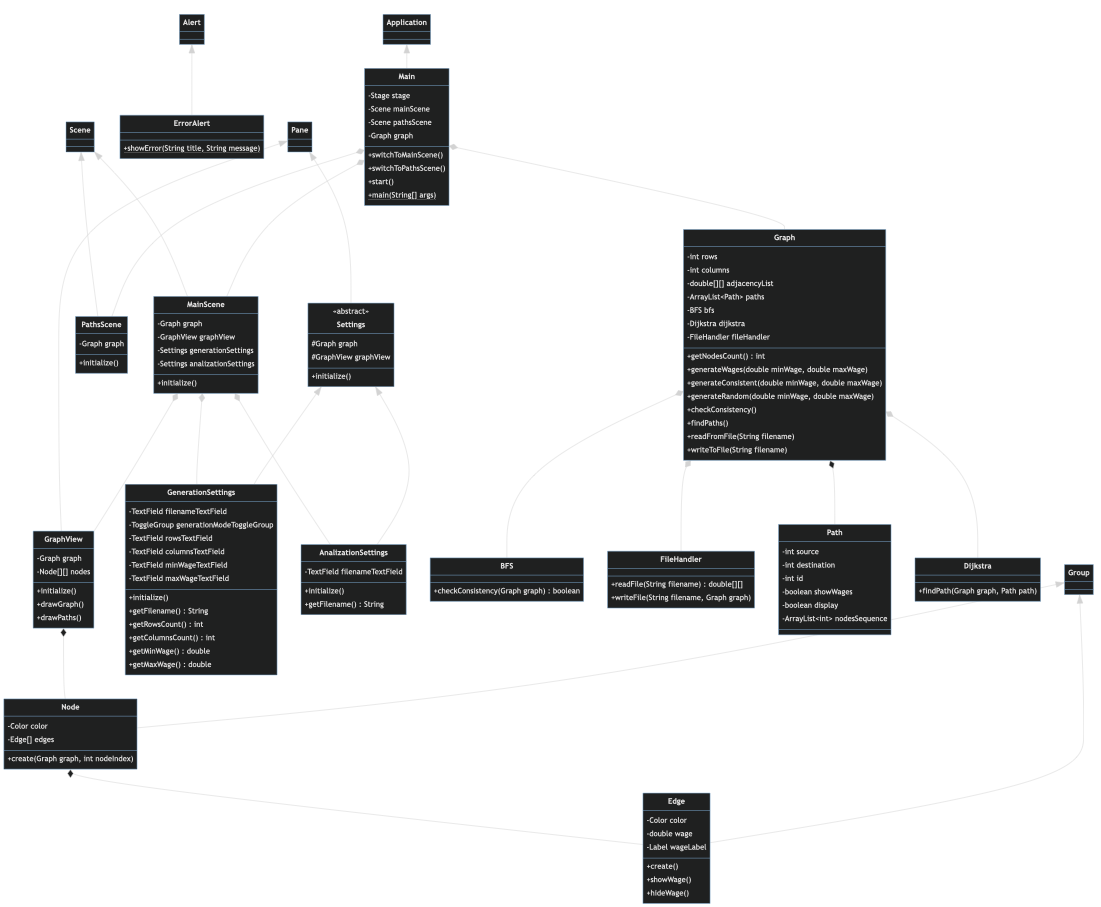
\includegraphics[width=15cm]{images/class_diagram.png}
        \caption{Klasy składające się na program oraz powiązania między nimi}
        \label{fig:class_diagram}
\end{figure}

\newpage

\subsection{Opis klas}
W tej sekcji znajdują się opisy klas oraz atrybutów i metod w nich zawartych.
\begin{itemize}
    \item \textbf{Main} -- wejście do programu. Startuje aplikacją i przechowuje referencje do scen i grafu.
    
    Atrybuty:
    \begin{itemize}
        \item \textbf{Stage stage} -- okno aplikacji,
        \item \textbf{Scene mainScene} -- główna scena aplikacji,
        \item \textbf{Scene pathsScene} -- scena edycji ścieżek,
        \item \textbf{Graph graph} -- referencja do obiektu reprezentującego graf.
    \end{itemize}
    
    Metody:
    \begin{itemize}
        \item \textbf{switchToMainScene()} -- przełącza do głównej sceny programu,
        \item \textbf{switchToPathsScene()} -- przełącza do sceny edycji ścieżek,
        \item \textbf{start()} -- inicjalizuje aplikację,
        \item \textbf{main(String[ ] args)} -- stanowi wejście do programu.
    \end{itemize}
    
    \item \textbf{ErrorAlert} -- statyczna klasa służąca do pokazywania komunikatów\linebreak o błędach.
    
    Metody:
    \begin{itemize}
        \item \textbf{showError(String title, String message)} -- pokazuje alert o zadanym tytule i treści.
    \end{itemize}
    
    \item \textbf{PathsScene} -- klasa stanowiąca scenę do zarządzania ścieżkami.
    
    Atrybuty:
    \begin{itemize}
        \item \textbf{Graph graph} -- referencja do obiektu reprezentującego graf.
    \end{itemize}
    
    Metody:
    \begin{itemize}
        \item \textbf{initialize()} -- inicjalizuje scenę.
    \end{itemize}
    
\newpage
    
    \item \textbf{MainScene} -- klasa stanowiąca scenę główną programu.
    
    Atrybuty:
    \begin{itemize}
        \item \textbf{Graph graph} -- referencja do obiektu reprezentującego graf,
        \item \textbf{GraphView graphView} -- referencja do obiektu reprezentującego sekcję GUI z narysowanym grafem,
        \item \textbf{Settings generationSettings} -- referencja do obiektu reprezentującego sekcję GUI z opcjami do generowania grafu,
        \item \textbf{Settings analizationSettings} -- referencja do obiektu reprezentującego sekcję GUI z opcjami do analizowania grafu.
    \end{itemize}
    
    Metody:
    \begin{itemize}
        \item \textbf{initialize()} -- inicjalizuje scenę.
    \end{itemize}
    
    \item \textbf{Settings} -- \emph{abstrakcyjna} klasa stanowiąca reprezentację sekcji z opcjami.
    
    Atrybuty:
    \begin{itemize}
        \item \textbf{Graph graph} -- referencja do obiektu reprezentującego graf,
        \item \textbf{GraphView graphView} -- referencja do obiektu reprezentującego sekcję GUI z narysowanym grafem.
    \end{itemize}
    
    Metody:
    \begin{itemize}
        \item \textbf{initialize()} -- inicjalizuje sekcję.
    \end{itemize}
    
    \item \textbf{AnalizationSettings} -- klasa stanowi reprezentację sekcji z opcjami\linebreak do analizowania grafu.
    
    Atrybuty:
    \begin{itemize}
        \item \textbf{TextField filenameTextField} -- referencja do obiektu reprezentującego pole tekstowe z nazwą pliku wejściowego.
    \end{itemize}
    
    Metody:
    \begin{itemize}
        \item \textbf{initialize()} -- inicjalizuje sekcję,
        \item \textbf{getFilename() : String} -- zwraca nazwę pliku wpisaną do pola tekstowego.
    \end{itemize}
    
\newpage
    
    \item \textbf{GenerationSettings} -- klasa stanowi reprezentację sekcji z opcjami\linebreak do generowania grafu.
    
    Atrybuty:
    \begin{itemize}
        \item \textbf{TextField filenameTextField} -- referencja do obiektu reprezentującego pole tekstowe z nazwą pliku wyjściowego,
        \item \textbf{ToggleGroup generationModeToggleGroup} -- referencja do obiektu reprezentującego grupę pól typu radio, które służą do wyboru trybu generowania grafu,
        \item \textbf{TextField rowsTextField} -- referencja do obiektu reprezentującego pole tekstowe z liczbą wierszy,
        \item \textbf{TextField columnsTextField} -- referencja do obiektu reprezentującego pole tekstowe z liczbą kolumn,
        \item \textbf{TextField minWageTextField} -- referencja do obiektu reprezentującego pole tekstowe z minimalną wagą krawędzi,
        \item \textbf{TextField maxWageTextField} -- referencja do obiektu reprezentującego pole tekstowe z maksymalną wagą krawędzi.
    \end{itemize}
    
    Metody:
    \begin{itemize}
        \item \textbf{initialize()} -- inicjalizuje sekcję,
        \item \textbf{getFilename() : String} -- zwraca nazwę pliku wpisaną do pola tekstowego,
        \item \textbf{getRowsCount() : int} -- zwraca liczbę wierszy wpisaną do pola tekstowego,
        \item \textbf{getColumnsCount() int} -- zwraca liczbę kolumn wpisaną do pola tekstowego,
        \item \textbf{getMinWage() : double} -- zwraca minimalną wagę krawędzi wpisaną do pola tekstowego,
        \item \textbf{getMaxWage() : double} -- zwraca maksymalną wagę krawędzi wpisaną do pola tekstowego.
    \end{itemize}
    
\newpage
    
    \item \textbf{GraphView} -- klasa stanowi reprezentację sekcji z widokiem wczytanego lub wygenerowanego grafu.
    
    Atrybuty:
    \begin{itemize}
        \item \textbf{Graph graph} -- referencja do obiektu reprezentującego graf,
        \item \textbf{Node[ ][ ] nodes} -- pole reprezentujące wierzchołki grafu (GUI).
    \end{itemize}
    
    Metody:
    \begin{itemize}
        \item \textbf{initialize()} -- inicjalizuje sekcję,
        \item \textbf{drawGraph()} -- rysuje graf na podstawie jego definicji,
        \item \textbf{drawPaths()} -- rysuje ścieżki na podstawie ich definicji.
    \end{itemize}
    
    \item \textbf{Node} -- klasa stanowi reprezentację wierzchołka grafu (GUI).
    
    Atrybuty:
    \begin{itemize}
        \item \textbf{Color color} -- pole przechowujące kolor wierzchołka,
        \item \textbf{Edge[ ] edges} -- pole reprezentujące krawędzie wychodzące z danego wierzchołka (GUI).
    \end{itemize}
    
    Metody:
    \begin{itemize}
        \item \textbf{create(Graph graph, int nodeIndex)} -- tworzy graficzną reprezentację danego wierzchołka grafu.
    \end{itemize}
    
    \item \textbf{Edge} -- klasa stanowi reprezentację wierzchołka grafu (GUI).
    
    Atrybuty:
    \begin{itemize}
        \item \textbf{Color color} -- pole przechowujące kolor krawędzi,
        \item \textbf{double wage} -- wartość wagi krawędzi,
        \item \textbf{Label wageLabel} -- referencja do obiektu reprezentującego etykietę z napisem zawierającym wartość wagi krawędzi.
    \end{itemize}
    
    Metody:
    \begin{itemize}
        \item \textbf{create()} -- tworzy graficzną reprezentację danej krawędzi grafu,
        \item \textbf{showWage()} -- wyświetla wagę dla krawędzi,
        \item \textbf{hideWage()} -- ukrywa wagę dla krawędzi.
    \end{itemize}
    
\newpage
    
    \item \textbf{Graph} -- klasa stanowi reprezentację grafu.
    
    Atrybuty:
    \begin{itemize}
        \item \textbf{int rows} -- liczba wierszy grafu,
        \item \textbf{int columns} -- liczba kolumn grafu,
        \item \textbf{double[ ][ ] adjacencyList} -- graf przechowywany jako lista sąsiedztwa,
        \item \textbf{ArrayList$<$Path$>$ paths} -- lista przechowująca ścieżki,
        \item \textbf{BFS bfs} -- referencja do obiektu implementującego algorytm BFS,
        \item \textbf{Dijkstra dijkstra} -- referencja do obiektu implementującego algorytm Dijkstry,
        \item \textbf{FileHandler fileHandler} -- referencja do obiektu obsługującego zapis i odczyt plików.
    \end{itemize}
    
    Metody:
    \begin{itemize}
        \item \textbf{getNodesCount() : int} -- zwraca liczbę wierzchołków grafu,
        \item \textbf{generateWages(double minWage, double maxWage)} -- generuje graf ze wszystkimi krawędziami i wagami losowymi w zadanym przedziale,
        \item \textbf{generateConsistent(double minWage, double maxWage)} -- generuje graf spójny z wagami losowymi w zadanym przedziale,
        \item \textbf{generateRandom(double minWage, double maxWage)} -- generuje graf w pełni losowy z wagami losowymi w zadanym przedziale,
        \item \textbf{checkConsistency()} -- sprawdza spójność grafu,
        \item \textbf{findPaths()} -- szuka najkrótszych ścieżek w grafie na podstawie ich definicji,
        \item \textbf{readFromFile(String filename)} -- wczytuje graf z pliku o zadanej nazwie,
        \item \textbf{writeToFile(String filename)} -- zapisuje graf do pliku o zadanej nazwie.
    \end{itemize}
    
\newpage
    
    \item \textbf{Path} -- klasa opisuje ścieżkę między dwoma wierzchołkami grafu.
    
    Atrybuty:
    \begin{itemize}
        \item \textbf{int source} -- numer wierzchołka źródłowego,
        \item \textbf{int destination} -- numer wierzchołka docelowego,
        \item \textbf{int id} -- numer identyfikacyjny ścieżki,
        \item \textbf{boolean showWages} -- czy pokazywać wagi dla przejść między wierzchołkami grafu,
        \item \textbf{boolean display} -- czy wyświetlać ścieżkę,
        \item \textbf{ArrayList$<$int$>$ nodesSequence} -- sekwencja numerów wierzchołków od wierzchołka źródłowego do docelowego.
    \end{itemize}
    
    \item \textbf{FileHandler} -- klasa służąca do obsługi plików.
    
    Metody:
    \begin{itemize}
        \item \textbf{readFile(String filename) : double[ ][ ]} -- wczytuje graf z pliku o zadanej nazwie,
        \item \textbf{writeFile(String filename, Graph graph)} -- zapisuje dany graf do pliku o zadanej nazwie.
    \end{itemize}
    
    \item \textbf{BFS} -- klasa służąca do analizy grafu pod kątem spójności.
    
    Metody:
    \begin{itemize}
        \item \textbf{checkConsistency(Graph graph) : boolean} -- analizuje spójność grafu z wykorzystaniem algorymtu BFS.
    \end{itemize}
    
    \item \textbf{Dijkstra} -- klasa służąca do wyszukiwania najkrótszej ścieżki między zadanymi wierzchołkami w grafie.
    
    Metody:
    \begin{itemize}
        \item \textbf{findPath(Graph graph, Path path)} -- wyszukuje najkrótszą ścieżkę w grafie dla zadanych wierzchołków przy użyciu algorymtu Dijkstry.
    \end{itemize}
\end{itemize}

\newpage

\section{Środowisko programistyczne}
Elementy wchodzące w skład środowiska programistycznego, w którym powstawał prorgram zostały wypisane poniżej.
\begin{itemize}
    \item Maszyna wirtualna języka Java (JVM): \textbf{Java SE 8}.
    \item Wersja oprogramowania developerskiego (JDK): \textbf{OpenJDK 1.8}
    \item System operacyjny: \textbf{Windows 10, macOS Monterey 12.2}.
    \item System kontroli wersji: \textbf{Git 2.34.1}.
    \item IDE: \textbf{IntelliJ IDEA 2021.3.2}.
    
\end{itemize}

\section{Praca z repozytorium}
Poniżej zostały przedstawione przyjęte konwencje w odniesieniu do pracy z repozytorium. 
\begin{itemize}
    \item Projekt wykorzystuje system kontroli wersji \textbf{Git}.
    \item Każdy moduł będzie tworzony na osobnej gałęzi.
    \item Nazwy gałęzi odzwierciedlają nazwy modułów z dopiskiem \textbf{"\textunderscore java"}\linebreak (np. moduł \emph{graph} jest tworzony na gałęzi o nazwie \emph{graph\textunderscore java})
    \item Jeżeli pojawi się potrzeba utworzenia gałęzi, która nie jest związana \linebreak w sposób jednoznaczny z modułem, to taka czynność jest dozwolona \linebreak(w tym wypadku nazwa gałęzi jest dowolna).
    \item Po ukończeniu prac implementacyjnych nad danym modułem jego gałąź będzie łączona z gałęzią główną.
    \item Dopuszcza się jednak pojedyncze commity tworzone bezpośrednio na gałęzi głównej, jeśli zajdzie taka potrzeba.
    \item Komentarze, jakimi opatrywane są commity, są dowolne (nie ma narzuconej żadnej konwencji pisania komentarzy).
\end{itemize}

\section{Konwencje nazewnicze}
Wszystkie konwencje nazewnicze są zgodne z ogólnymi zasadami pisania kodu w języku Java przyjętymi przez jej społeczność.

\newpage

\section{Testy programu}

Kod będzie testowany za pomocą automatycznych testów jednostkowych napisanych przy pomocy biblioteki \textbf{JUnit}. Wszystkie pliki potrzebne przy testowaniu znajdują się w katalogu zawierającym testy jednostkowe.
\subsection{Pliki testowe}
Poniżej zostały przedstawione pliki wykorzystywane w testach programu.\\
\noindent Pliki:
\begin{itemize}
    \item \emph{t\textunderscore graph.txt} (\emph{Rysunek \ref{fig:wagi}}) -- przechowuje graf o wymiarach \textbf{4 x 4} z wszystkimi krawędziami i wagami.
\begin{lstlisting}
4 4
	 1 :0.3  4 :0.2 
	 5 :0.2  2 :0.6  0 :0.4 
	 6 :0.8  3 :0.4  1 :0.6
	 7 :0.5  2 :0.8 
	 8 :0.9  0 :0.8  5 :0.9 
	 1 :0.5  9 :0.3  6 :0.4  4 :0.4 
	 10 :0.7  7 :0.7  2 :0.2  5 :0.3 
	 6 :0.9  3 :0.7  11 :0.7 
	 4 :0.7  12 :0.5  9 :0.2 
	 13 :0.8  5 :0.8  8 :0.4  10 :0.4 
	 14 :0.5  6 :0.5  9 :0.7  11 :0.3 
	 15 :0.3  10 :0.6  7 :0.8 
	 13 :0.5  8 :0.5 
	 9 :0.7  12 :0.7  14 :0.4 
	 10 :0.8  15 :0.2  13 :0.2 
	 11 :0.7  14 :0.4 
\end{lstlisting}
\begin{figure}[htp]
    \centering
    \includegraphics[width=6cm]{images/wagi.png}
    \caption{Wizualizacja pliku \emph{t\textunderscore graph.txt}}
    \label{fig:wagi}
\end{figure}
\item \emph{cos\textunderscore graph.txt} -- przechowuje graf spójny. Jest modyfikacją grafu z pliku \emph{t\textunderscore graph.txt}, w którym nie istnieje krawędź między wierzchołkami \textbf{15 i 11}.
\begin{lstlisting}
4 4
	 1 :0.3  4 :0.2 
	 5 :0.2  2 :0.6  0 :0.4 
	 6 :0.8  3 :0.4  1 :0.6
	 7 :0.5  2 :0.8 
	 8 :0.9  0 :0.8  5 :0.9 
	 1 :0.5  9 :0.3  6 :0.4  4 :0.4 
	 10 :0.7  7 :0.7  2 :0.2  5 :0.3 
	 6 :0.9  3 :0.7  11 :0.7 
	 4 :0.7  12 :0.5  9 :0.2 
	 13 :0.8  5 :0.8  8 :0.4  10 :0.4 
	 14 :0.5  6 :0.5  9 :0.7  11 :0.3 
	 10 :0.6  7 :0.8 
	 13 :0.5  8 :0.5 
	 9 :0.7  12 :0.7  14 :0.4 
	 10 :0.8  15 :0.2  13 :0.2 
	 14 :0.4 
\end{lstlisting}
\item \emph{incos\textunderscore graph.txt} -- przechowuje graf niespójny. Jest modyfikacją grafu z pliku \emph{t\textunderscore graph.txt}, w którym wierzchołek \textbf{11} nie jest połączony z żadnym innym wierzchołkiem.
\begin{lstlisting}
4 4
	 1 :0.3  4 :0.2 
	 5 :0.2  2 :0.6  0 :0.4 
	 6 :0.8  3 :0.4  1 :0.6
	 7 :0.5  2 :0.8 
	 8 :0.9  0 :0.8  5 :0.9 
	 1 :0.5  9 :0.3  6 :0.4  4 :0.4 
	 10 :0.7  7 :0.7  2 :0.2  5 :0.3 
	 6 :0.9  3 :0.7  
	 4 :0.7  12 :0.5  9 :0.2 
	 13 :0.8  5 :0.8  8 :0.4  10 :0.4 
	 14 :0.5  6 :0.5  9 :0.7   
	  
	 13 :0.5  8 :0.5 
	 9 :0.7  12 :0.7  14 :0.4 
	 10 :0.8  15 :0.2  13 :0.2 
	 14 :0.4 
\end{lstlisting}

\newpage

\item \emph{wf\textunderscore graph.txt} - przechowuje graf zapisany w nieprawidłowym formacie. Nieprawidłowy format w tym przypadku polega na tym, że w pierwszej linii pliku oprócz wymiarów grafu znajdują się informacje o wierzchołkach sąsiadujących.
\begin{lstlisting}
4 4 1 :0.3  4 :0.2 
	1. 5 :0.2  2 :0.6  0 :0.4 
	2. 6 :0.8  3 :0.4  1 :0.6
	3. 7 :0.5  2 :0.8 
	4. 8 :0.9  0 :0.8  5 :0.9 
	5. 1 :0.5  9 :0.3  6 :0.4  4 :0.4 
	6. 10 :0.7  7 :0.7  2 :0.2  5 :0.3 
	 6 :0.9  3 :0.7  11 :0.7 
	 4 :0.7  12 :0.5  9 :0.2 
	 13 :0.8  5 :0.8  8 :0.4  10 :0.4 
	 14 :0.5  6 :0.5  9 :0.7  11 :0.3 
	 15 :0.3  10 :0.6  7 :0.8 
	 13 :0.5  8 :0.5 
	 9 :0.7  12 :0.7  14 :0.4 
	 10 :0.8  15 :0.2  13 :0.2 
	 11 :0.7  14 :0.4 
\end{lstlisting}

\end{itemize}


\end{document}
